The verification platform is organized as a closed-loop flow that combines pre-generated test cases, FPGA-side verification, and PC-side result analysis. The overall structure of this verification platform is presented in Figure~\ref{fig:verification_platform}. In this work, the $3 \times 3$ mesh NoC is treated as the design under test (DUT). Test cases are first generated on the host computer and encoded into a ROM initialization file. During execution, the test controller fetches packet entries from the initialized ROM, and the generator injects the corresponding packets into the DUT. The received packets are checked on chip, and the verification results are reported back to the host computer through UART.

\begin{figure}[htbp]
    \centering
    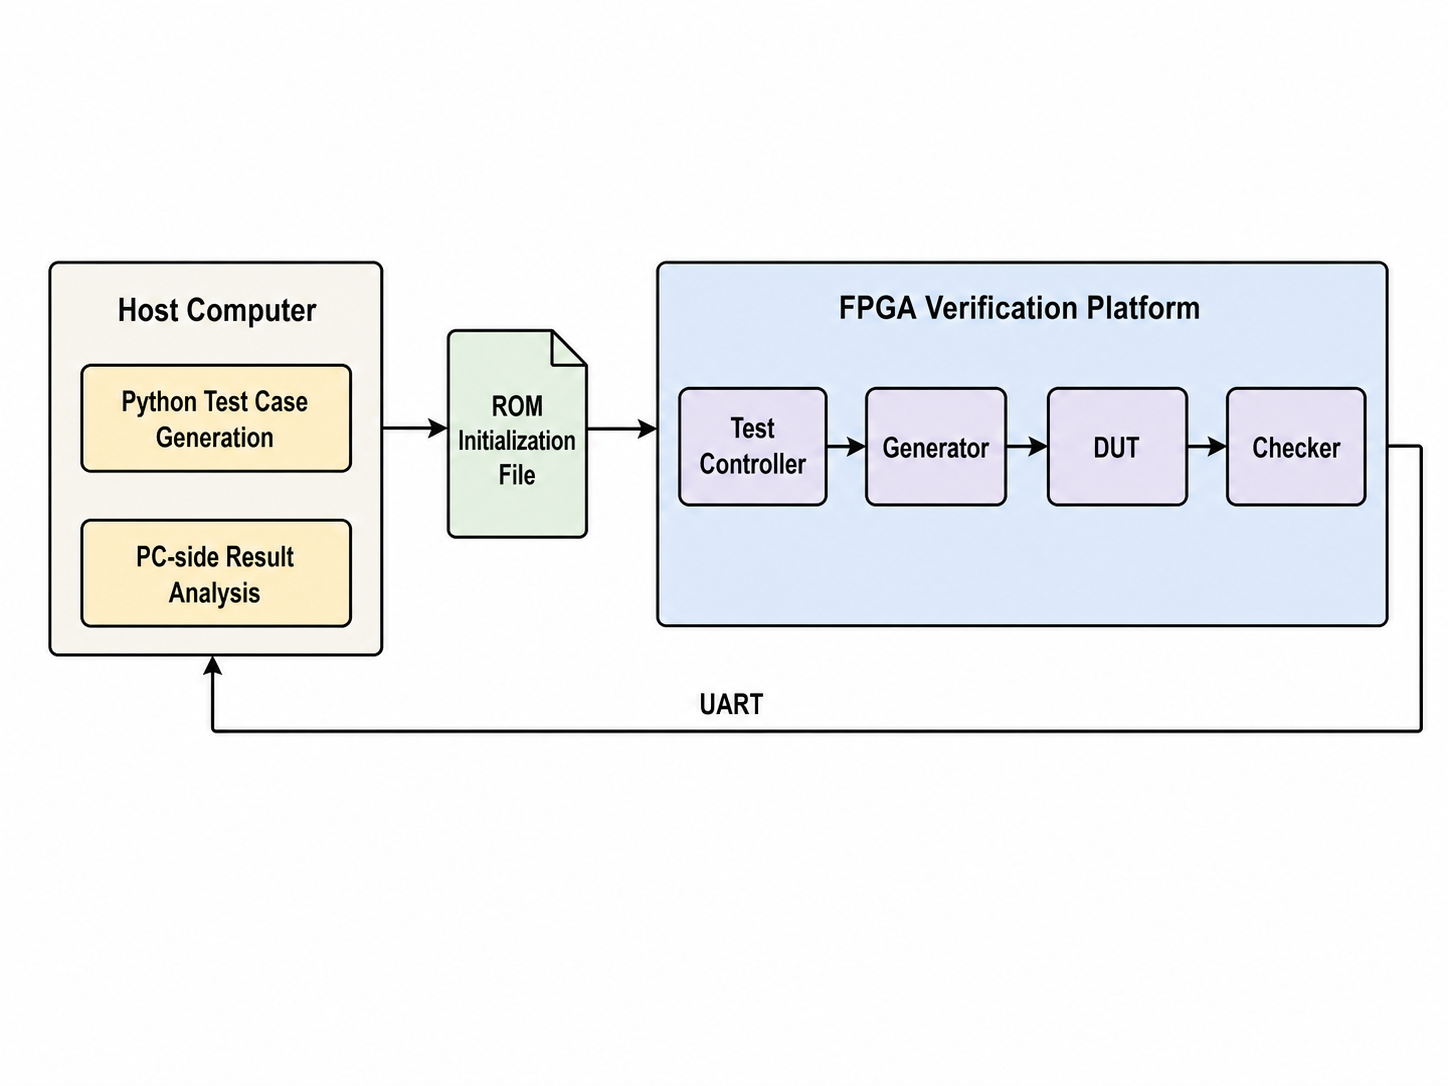
\includegraphics[width=0.9\textwidth]{images/ch4_verification_and_results/overall_platform.png}
    \caption{Overall verification platform}
    \label{fig:verification_platform}
\end{figure}
